\documentclass[]{article}

% Packages/Macros
\usepackage{amssymb}
\usepackage{latexsym}
\usepackage{amsmath}
\usepackage{graphicx}
\usepackage{fixltx2e}
\usepackage[letterpaper,left=1in,right=1in,top=0.8in,bottom=0.8in,footskip=0.25in]{geometry}
\usepackage{color}
\usepackage{subcaption}
\usepackage{float}
\usepackage{tikz}
\usetikzlibrary{matrix,shapes,arrows,positioning,chains}
\usepackage{hyperref}
\hypersetup{colorlinks=true,urlcolor=blue,linkcolor=blue}
\usepackage{listings}

% Document
\begin{document}

\title{\vspace{-10mm}An Analysis Pathway for Methylation Data}
\author{Pavel Komarov}
\maketitle
  
  \section{Introduction}
  In the end, we hope to gain an understanding of how genomic methylation may deviate from normal in Schizophrenia patients. We take a heavily data-driven and algorithmic approach, attempting to elucidate the \href{http://www.ncbi.nlm.nih.gov/geo/query/acc.cgi?acc=GSE74193}{data} in a way its generators [\ref{r:jaffe}] did not. We hope the methods and expertise we develop in this process are reusable on different, better data in the future and might enable us to answer important questions like ``Can we diagnose a disease with epigenetic data?'' or ``Can we identify a complex combination of factors that might be causing or correlated with a disease?'', questions we might otherwise find intractible.

  \section{Data Flow}

  Immediately after the questions ``What are we doing?'' and ``Why are we doing it?'' comes ``How?''. In the case of this project, how is with a datapath. In order to understand our investigation precisely and be able to replicate or expand the results, it is essential to understand the data transformations shown below.

  \subsection{A Diagram of the process}
  \vspace{2mm}

  % Define block styles
  \tikzstyle{file} = [rectangle, text width=10em, inner sep=0pt]
  \tikzstyle{unit} = [rectangle, draw, text centered, minimum height=1.5em]
  \tikzstyle{notes} = [rectangle, scale=0.8, text width=10em]
  \tikzstyle{line} = [draw, -latex']

  \begin{center} \begin{tikzpicture}[node distance = 1cm, auto]
    % Place nodes
    \node [file] at (0,0) (0_GSE) {0\_GSE74193\_GEO\_procData.csv};
    \node [notes] at (1.6,-0.4) (gse_notes) {$\dagger$correct loci?};
    \node [file] at (5.5,0) (0_Probes) {0\_Probes\_to\_exclude\_64410.txt};
    \node [file] at (10.5,0) (0_meta) {0\_jaffe\_metadata.csv};
    
    \node [unit] at (0,-1.5) (JaffeParser) {JaffeParser.java};
    \node [notes] at (0.2,-2.3) (parser_notes) {*tweak \newline $\dagger$what to exclude as NA?};
    \node [file] at (4.5,-1.8) (1_processed) {1\_processed\_SZ\_vs\_control.csv \newline 1\_processed\_SZ\_vs\_youth.csv \newline 1\_processed\_control\_vs\_youth.csv};
    \node [unit] at (10,-1.5) (MetaMatcher) {MetaMatcher.java};
    \node [file] at (10,-3) (1_meta) {1\_metadata\_SZ\_vs\_control.csv \newline 1\_metadata\_SZ\_vs\_youth.csv \newline 1\_metadata\_control\_vs\_youth.csv};

    \node [unit] at (0,-4) (GetResiduals) {GetResiduals.R};
    \node [notes] at (0.2,-5) (gr_notes) {*tweak \newline *run in PACE \newline $\dagger$what sort of model to use?};
    \node [file] at (4,-4) (2_resids) {2\_residuals\_SZ\_vs\_control.csv \newline 2\_residuals\_SZ\_vs\_youth.csv \newline 2\_residuals\_control\_vs\_youth.csv};
    \node [unit] at (10,-4.5) (Construct) {ConstructSPDData.m};
    \node [notes] at (9.7,-5) (constr_notes) {*tweak};

    \node [unit] at (0.9,-6.3) (PC) {GetPrincipleComponents.R};
    \node [notes] at (0.2,-7.2) (PC_notes) {*PACE \newline $\dagger$what do with \newline NAs?};
    \node [unit] at (5.8,-6.3) (Iso) {Isomap.R};
    \node [notes] at (5.8,-7.2) (PC_notes) {*PACE \newline $\dagger$what do \newline with NAs?};
    \node [file] at (10,-6.7) (spdmats) {SZ\_vs\_control.mat \newline SZ\_vs\_youth.mat \newline control\_vs\_youth.mat \newline SZ\_vs\_control\_resid.mat \newline SZ\_vs\_youth\_resid.mat \newline control\_vs\_youth\_resid.mat};  

    \node [file] at (0.9,-8.5) (resid_PCs) {$\triangleright$pcs\_all.png \newline $\triangleright$pcs\_top\_20.png \newline 3\_residPCs\_SZ\_vs\_control.csv};
    \node [file] at (5.8,-8.5) (residisos) {$\triangleright$isos2.png \newline $\triangleright$Rplots.pdf \newline 3\_residiso\_k2\_SZ\_vs\_control.csv};

    \node [unit] at (3.5,-10) (classify) {classify.py};
    \node [notes] at (3.7,-10.7) (classnotes) {*tweak \newline $\dagger$what k?};
    \node [unit] at (10,-10) (spd) {progression\_GUI.m};

    \node [file] at (3.5,-11.8) (classouts) {$\triangleright$a plot in python \newline $\ddagger$the ability to classify new data};
    \node [file] at (10,-11.5) (spdouts) {more .mat files};

    % Draw edges
    \path [line] (0_GSE) -- (JaffeParser);
    \path [line] (0_meta) |- ([yshift=5mm] JaffeParser.north) -- (JaffeParser);
    \path [line] (0_Probes) |- ([yshift=5mm] JaffeParser.north) -- (JaffeParser);
    
    \path [line] (JaffeParser) -| ([xshift=-5mm] 1_processed.west) -- (1_processed);
    \path [line] ([xshift=2mm] 0_meta.south) |- ([yshift=3mm] MetaMatcher.north) -- (MetaMatcher);
    \path [line] ([xshift=10mm] 1_processed.east) -| ([xshift=-7mm] MetaMatcher.west) -- (MetaMatcher);
    \path [line] (MetaMatcher) -- (1_meta);
    
    \path [line] (1_processed) |- ([yshift=7.3mm] GetResiduals.north) -- (GetResiduals);
    \draw (1_meta) -| ([yshift=-6mm] 1_processed.south);
    \path [line] (GetResiduals) -- (2_resids);
    \path [line] (1_meta) -- (Construct);
    \path [line] ([xshift=1cm] 2_resids.east) -| ([xshift=-3mm] Construct.west) -- (Construct);

    \path [line] (2_resids) |- ([yshift=3mm] PC.north) -- (PC);
    \path [line] (2_resids) |- ([yshift=3mm] Iso.north) -- (Iso);
    \path [line] (Construct) -- (spdmats);

    \path [line] (PC) -- (resid_PCs);
    \path [line] (Iso) -- (residisos);
    \path [line] (spdmats) -- (spd);

    \path [line] (resid_PCs) |- ([yshift=3mm] classify.north) -- (classify);
    \path [line] (residisos) |- ([yshift=3mm] classify.north) -- (classify);

    \path [line] (classify) -- (classouts);
    \path [line] (spd) -- (spdouts);

  \end{tikzpicture} \end{center}

  \subsection{How to read the diagram}
  Boxed items are ``units'', pieces of code made for processing things (located in \texttt{/code}). Unboxed text represents files (located in \texttt{/data}). I've prefixed datasets with numbers to roughly indicate their stage in the process. Outputs prefixed by a $\triangleright$ are side-effects intended to give some insight in to what just happened. Smaller text under units or files are ``notes''. Those beginning with * are directions for use: ``PACE'' means ``This unit should be run in the cluster if you want it to finish.''; ``tweak'' means ``You will have to modify the actual text of the unit (and sometimes then recompile) to make it generate different outputs.'' Notes beginning with $\dagger$ are essential questions that plague us. If they appear below a unit, I had to find an answer in order to create that unit. You should know that my solutions to these problems---in all cases---are not necessarily right, but I spent a great deal of time trying to understand the issues and ensuring my answers were at least good. I make a few arguments for my choices in this document as well as in code comments.

  \section{Stepwise instructions for how to do what the diagram shows + What things are and mean}
  \subsection{Preliminaries}
  We begin with the 0s: \texttt{GSE74193\_GEO\_procData.csv} is directly from Jaffe, et al.; \texttt{jaffe\_metadata.csv} is created by passing a minorly-modified \texttt{GSE74193\_series\_matrix.tsv} through \texttt{CSVTransposer.java}; and \texttt{Probes\_to\_exclude\_64410.txt} is made by joining a couple of other exclusion lists together without duplicates.

  I find it most convenient to interact with \texttt{.csv} files through a program like LibreOffice or Excel, since they can put the comma-separated data in cells and make it more readable. But do not try to open large datasets with these programs, or your computer will run out of memory and freeze. LibreOffice's `text import' screen (that appears when opening \texttt{.csv}s) is nice because it gives a preview of the data without trying to read all of it, so the schema is visible. \texttt{more <filename>} on the command line can be used to print large files piece by piece, not as neat as an office-type program but often equally as effective.

  \subsection{Basic processing}
  At stage 1 I take all 0s as inputs to \texttt{JaffeParser.java} and output what I call ``processed'' data. That is: Exclude all the probes listed in the exclude file; set all ``beta'' methylation values with a corresponding p value $>0.05$ to be \texttt{NA}; exclude samples from plate 244 (known to suffer from exceptionally bad batch effects); only include the best samples from each subject; and only include the subjects who meet certain criteria (like exceed some age or have a certain disease state). Note that this last distinction is the difference between the three outputs of this unit.

  To use the \texttt{JaffeParser}, first modify the subject-inclusion criteria on lines 42-47. Then recompile with \texttt{javac JaffeParser.java}, and run with \texttt{java JaffeParser <data> <metadata> <excludelist> <out>}, where everything labelled with $<>$ is replaced by literal file paths. Next run the \texttt{MetaMatcher} with \texttt{java MetaMatcher <data> <metadata> <out>} to generate cleaned-up metadata files corresponding perfectly to the datasets generated by the parser.

  \subsection{Getting rid of everything that isn't disease state}
  At stage 2 I generate what I term the ``flattened'' datasets by passing the processed data and metadata to \texttt{GetResiduals.R}. The computation is done in the cluster because it takes loads of memory and can crash your system (as it did mine several times). Open your root directory in PACE and make sure \texttt{GetResiduals.R} is in a subdirectory called \texttt{/code}. Open this R file and make sure that it is looking for \texttt{.csv} files that exist in the \texttt{/data} subdirectory. Then \texttt{ssh} in to PACE and submit the job with \texttt{msub GetResiduals.pbs}. If that didn't make perfect sense, see Section \ref{cluster} where I've laid out some details.

  Conceptually, this step fits a linear model to explain why the data varies as it does according to the Sex, Age, and Ethnicity of individuals, the four PCs that best characterize batch effects (provided by Jaffe, et al. in the metadata), and the cellular composition of samples (embrionic stem, dopaminergic neuron, et cetera). Once a fit is computed, the script subtracts this fit from the real data and returns the difference, termed the ``residuals''. This leftover variation is unexplained by the model, or in other words may be due to causes not accounted for in the model. But a few problems arise here: What if a linear model is not the right choice so the leftovers we see are the artefacts of an intrinsically poor fit instead of an unseen cause (like disease state)? What if the leftover variation is small? Might it just be noise? How can we be sure?

  \begin{figure}[H]
    \centering
    \begin{subfigure}{.95\textwidth}
      \centering
      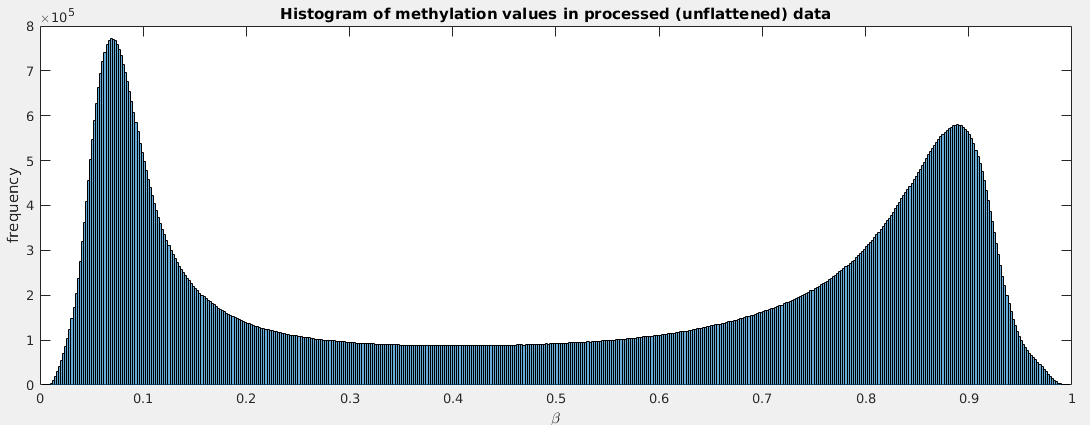
\includegraphics[width=1\linewidth]{hist1.png}
      \caption{processed}
    \end{subfigure}
    \begin{subfigure}{.95\textwidth}
      \centering
      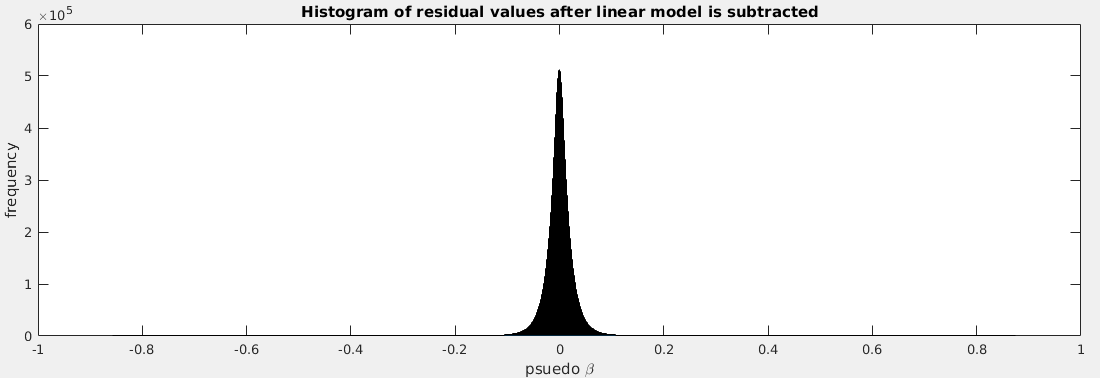
\includegraphics[width=1\linewidth]{hist2.png}
      \caption{flattened}
    \end{subfigure}
    \caption{Histograms of SZ\_vs\_control datasets (which include samples from Schizophrenic brains and controls over 16.)}
    \label{fig:hists}
  \end{figure}

  I hope Figure \ref{fig:hists} demonstrates in stark terms what this step has done and helps you recognize how to answer some of the questions posed above: After flattening, the leftover data is sharply centered around zero. It's basically a Dirac delta. Whereas before the values intuitively correspond to degrees of methylation at loci, the new values can be positive or negative depending upon whether the model was larger or smaller than the input data at a locus. This outcome means a few things: (1) Sex, Age, Ethnicity, et cetera explain most (if not all, considering noise) of the variation in the original dataset. (2) Because a linear model can match the processed data so closely as to return such small residuals, its characterization power of this dataset is at least very good. (3) There isn't much left to be explained by disease state, or there isn't much left to explain disease state (depending upon which way you think the arrow of causality goes).

  Whether the little bit of variation left is noise is still unclear. Ideally we would like the subtraction performed at this step to yield a fairly sharp, bimodal distribution, so we might clearly see a single divide the model could not explain yet be somewhat confident its characterization power was otherwise quite good. Since this is not the case, and since there is no simple mathematical or scientific proof that what remains is entirely noise, we need to rephrase the question. Let's pose it in engineering terms: Given the flattened data, can we build an agent that can distinguish between diseased and control at a better-than-random rate? If we can, then we have found some signal in the noise and can know that it is not all garbage.

  \subsection{Machine Learning: Definitions and how to approach the problem}

  We could try to be the agent ourselves or build some rule-based algorithm that can distinguish samples based on disease state, but the data is so large and conceptually inaccesssible that we need a different approach. Thankfully, we live in the age of Machine Learning.

  There are many classes of Machine Learning algorithm, and it is important to know what they are and what they do because: (1) Not every algorithm is suitable to every problem, and (2) the choice of algorithm has a large impact on how expensive training or querying will be.

  In the interest of making this document as practical as possible for you biologists, I include some explanations now.

  \begin{enumerate}
    \item \textit{Regression vs Classification} If we wish to assign some number from a continuous domain to each sample, then we should use regression; if we wish to assign one of a discrete set of answers to each sample, then we should use classification.

    \item \textit{Supervised vs Unsupervised} Supervised means we feed the algorithm $(x,y)$ pairs, where $x$ is the information we might see at query-time and $y$ is the answer we would have to find. The algorithm takes this input-output information and adjusts itself to increase the chance it outputs $y$ in the future given this $x$. It takes hundreds of thousands (if not millions) of pairs to create a generalizable model (one that is performant on data not included in the training set). Unsupervised means we don't have the answers to start with; all we know is that there may be some pattern in the data and and want to uncover it, with no regard (at least inside the algorithm) for what that pattern may mean.

    \item \textit{Parametric vs Instance} Parametric learners find a model that can be represented by a ``small'' set of parameters (i.e. much smaller than the size of the training data). In this paradigm, training takes a long time, there is no need to keep the training data around after training, and using the model is fast. Instance learners memorize and use the training data directly, which means training is fast, but the model is relatively large and querying it is slow.

    \item \textit{Batch vs Online} Batch learners train on a batch of data and must be completely retrained to accomodate any new information. Online learners do all their decision-making with query-time calculations, so incorporating new data doesn't involve a complete retrain.

    \item \textit{Generative vs Discriminative} A Generative learner seeks to find the ``generator'' function, the joint probability distribution of all input-output pairs: $P(x,y)$. If we know the generator function has a certain form, then this can be done easily with little data and then even be used to give us additional, simulated data. Discriminative learners are useful when we don't know what form the underlying model should have. They seek to find conditional probability distributions: $P(y|x)$. For example, a generative model might attempt to solve the problem ``Is this sentence in English or French?'' by trying to learn a theory of language that can model French and English with parameters, whereas a discriminative model would solve the problem by learning English and French and trying to fit any given sentence.
  \end{enumerate}

  To make these disctinctions concrete, let's review a few common algorithms with notes on their operation and how it determines their categorizations.

  \begin{itemize}
    \item \textit{K-Nearest Neighbors (kNN)} Training simply involves memorizing the data, and querying involves finding the $k$ most similar examples from training. This makes kNN an \textit{instance} learner. Including additional data does not require a retrain, so kNN is \textit{online}. kNN can either return some average or weighted combination of these $k$ training examples, in which case it would be doing \textit{regression}, or it can implement a voting-scheme and return only one \textit{classification}. kNN requires labels (answers) for each training point, so it is \textit{supervised}. And since kNN models the conditional probability of belonging to a class (discrete case) or of having a value on some domain (continuous case), it is \textit{discriminative}.
    \item \textit{Clustering} Combining things in to new classes based on their apparent similarity requires no knowledge of labels, so any form of clustering is \textit{unsupervised}. (Actually it's difficult to come up with an example of unsupervised learning that is \textit{not} some kind of clustering.) Clusters might end up different if we re-run the algorithm after including new points, in which case it would be \textit{batched}, or the algorithm might simply lump new points with the nearest cluster, in which case it might operate \textit{online}. The other distinctions listed do not apply.
    \item \textit{Neural Networks} Neural Nets are \textit{supervised}, requiring many training examples and thousands of rounds of backpropagation to tune. Backpropagation adjusts input weights of neurons, a set of numbers of a fixed size, the network's \textit{parameters}. A neural network can be trained \textit{online} if each new $(x,y)$ is used, but they are often simply trained on a \textit{batch} of data and then deployed without further adjustment. A network can do \textit{regression} if there is a single output neuron connected to the last hidden layer, but in practise a 1-of-$k$ \textit{classification} scheme often works better. For example, if you wanted to find a number between 0 and 9, you might have 10 output neurons and pass the number 5 as 0000010000 at the beginning of backpropagation, so that one neuron is trained to activate and the others to be silenced. As opposed to having to worry about how close the output is to some value, you can then interpret the intensity of the output on each of the 10 neurons as the network's confidence for each digit. Finally, Neural Nets are \textit{discriminative} because they find boundaries between classes instead of explicit models of joint probability.
  \end{itemize}

  So we have options (many more than listed), but which is the best option for gene microarray data? The short answer is it's difficult to know right away. And how do we even define ``best''? Does it mean fastest, most accurate, most ellucidating of some underlying pattern, most conceptually tractable?

  I've taken two main paths, one the easiest-to-understand classification scheme I could think of that does not require tens of thousands of training points (to answer the question ``Are these residuals just noise?'') and one based on pattern-finding, which is a bit more complicated. I will start with the first, and I begin that discussion with a preliminary issue: feature extraction.

  \subsection{Turning too many features in to something manageable}

  Let's make the concept of an $(x,y)$ pair more specific: An algorithm gets a load of information stacked in to a vector called $x$ and must find an output $y$ (often a single value). Elements of $x$ might be continuous (like a temperature measurement) or discrete (like a genre), but all can be mapped to numbers. If we call the length of $x$ $D$, then $x$ constitutes a point in $D$-dimensional space.

  In this hyperspace, the task of distinguishing known classes (supervised learning) becomes the task of drawing boundaries (hyper-surfaces) to divide groups of points with the same $y$ from each other, and a regression task becomes the task of finding some continuous function to describe $y$ throughout the space.

  Here's the rub: All methods to accomplish such jobs suffer from ``the curse of dimensionality''. That is, as the dimensionality of the input data $D$ grows, the computation and number of samples $N$ required to find a generalizable answer explodes.

  In our case we have a feature-space in 421103 dimensions (one for each CpG site after exclusions), far too large to work with, especially considering that (due to the high cost of biological experiments) our $N \sim100$. Note that this dimension is actually quite small in a biological sense since every individual has far, far more CpG sites. In the future we can expect both $D$ and $N$ to increase for this problem.

  The way to resolve this dilemma is by recognizing that not all these dimensions carry useful information, and some carry redundant information. So, intuitively, we should be able to recreate a somewhat faithful portrait of the data in a lower dimension, $d$, that captures its key elements. This is process of going from $N \times D$ to $N \times d$ is called ``feature reduction'', and to say it's a well-studied area is an understatement.

  As a consequence, many reduction methods have been developed. I used three: PCA, Isomap, and Hierarchical Clustering.

  \subsubsection{Principle Component Analysis}

  PCA is maybe the most common feature reduction method. It works as follows:

  \begin{lstlisting}[mathescape]
  1. Subtract the mean in every dimension and scale by the variance to get 
     adjusted data where features are more equally scaled.
  2. Calculate the covariance matrix $C$.
  3. Find eigenvalues, $\lambda$, and eigenvectors, $\vec{v}$, of $C$.
  4. Choose $n$ $\vec{v_{i}}$ with the largest corresponding $|\lambda_{i}|$. These are the PCs.
  5. $New\_data = adjusted\_data \cdot [\vec{v_{1}} \vec{v_{2}} ... \vec{v_{n}}]$
  \end{lstlisting}

  This isn't the only formulation of PCA---the method employed by R uses Singular Value Decomposition (SVD) to get the eigenthings---, but I think it gives a nice intuition. Essentially, you are looking for the vectors which best characterize the directions in which the data varies most, recording how much each datapoint varies in those directions, and throwing away all the other directions/dimensions.

  To accomplish this feature reduction on our data, I used R's \texttt{prcomp()} function and wrote a nice script to package it all up. To run it, put \texttt{GetPrincipleComponents.R} and \texttt{GetPrincipleComponents.pbs} in your \texttt{/code} subdirectory in PACE, make sure it's reading the right input file from \texttt{/data}, and submit the job (details in Section \ref{cluster}). Note that SVD and other methods of finding eigenvectors and -values do not work if there are \texttt{NA}s in the data, so I set them to be $0$ after centering and scaling the data. For a more complete discussion of this choice, see the comments in \texttt{GetPrincipleComponents.R}.

  PCA returns up to $N$ PCs, so PCA reduces the dimension from 21103 to 244 right away (in the case of SZ vs control), but most of the variance is usually captured in the top few PCs. Figure \ref{fig:pcvars} displays the variance in the direction of each PC across the $N$ samples.

  \begin{figure}[H]
    \centering
    \begin{subfigure}{.49\textwidth}
      \centering
      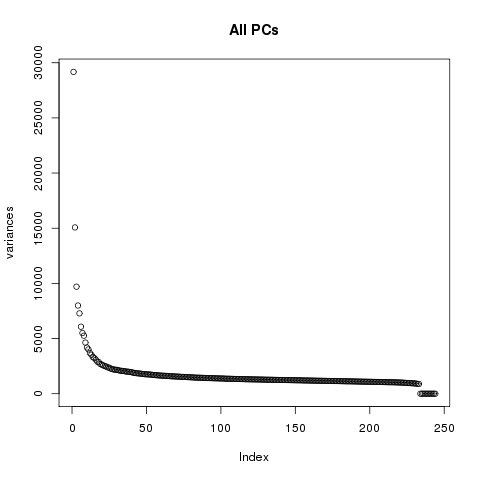
\includegraphics[width=1\linewidth]{pcs_all.png}
    \end{subfigure}
    \begin{subfigure}{.49\textwidth}
      \centering
      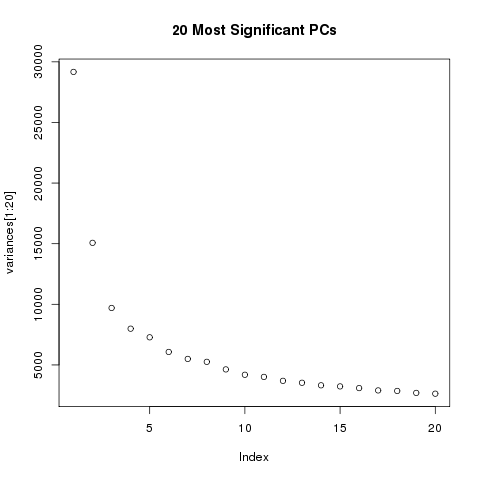
\includegraphics[width=1\linewidth]{pcs_top_20.png}
    \end{subfigure}
    \caption{Variance of the data in the direction of PCs.}
    \label{fig:pcvars}
  \end{figure}

  Notice that beyond some index, the curve flattens out. The PCs beyond this point contain comparatively little descriminative information, so if we wish to further reduce the dimension of the data (to make $N > d$), then we can ignore them.

  To make this clearer, Figure \ref{fig:pc3d} visualizes the samples as points in a space defined by the most-varying 3 PCs. Note that I've turned the figure to show the best separation I can, so it's not a perfectly honest measure, but some kind of difference between the groups appears to be visible. If you wish to generate this plot and play with it yourself, run \texttt{first3PCs.R}.

  \begin{figure}[H]
    \centering
    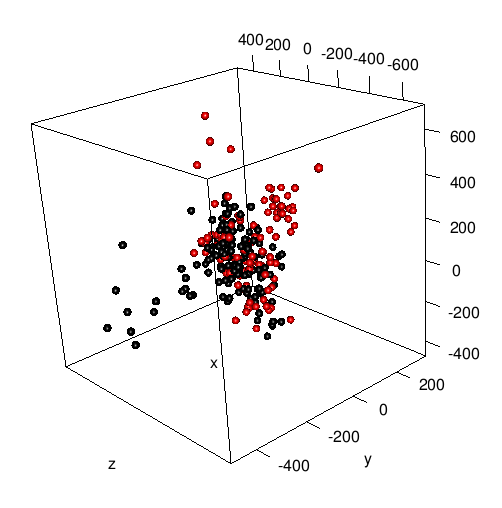
\includegraphics[width=0.7\linewidth]{pc3d.png}
    \caption{Visualization of Control samples (black) and SZ samples (red) in a space of the 3 most significant PCs.}
    \label{fig:pc3d}
  \end{figure}

  But there is a possible problem: PCA is inherently linear, so it can be terrible at discovering good features in highly nonlinear contexts. A common example is the ``swiss roll'' dataset shown in Figure 1 \href{https://www.bioconductor.org/packages/devel/bioc/vignettes/RDRToolbox/inst/doc/vignette.pdf}{here}. What if microarray data is nonlinear?

  \subsubsection{Isomap}

  Isomap is an increasingly popular way to characterize nonlinear data. Here is an outline:

  \begin{lstlisting}[mathescape]
  1. Construct a neighborhood graph as follows:
     for all ($x_{i},x_{j}$)
         if distance($x_{i},x_{j}$) $< \epsilon$
             add edge ($x_{i},x_{j}$) to G with weight 1
  2. Compute shortest distances along the graph edges $\delta_{G}(x_{i},x_{j})$ by Floyd-Warshall
  3. Apply multidimensional scaling to $\delta_{G}(x_{i},x_{j})$
  \end{lstlisting}

  Multidimensional scaling takes a set of things that all have set distances from each other (like graph edges) and tries to assign all of them locations in $d$-dimensional space such that these distances will be best preserved. I highly recommend Wikipedia's article for more details.

  But what you probably care more about is \texttt{Isomap.R}, an R script I have written to perform the above on our data utilizing the absurdly convenient \texttt{Isomap()} function from the \texttt{Bioconductor RDRToolbox} package. In order to get this to run, you will need to install that library in PACE (See instructions in Section \ref{adlib}), and then follow job submission steps analogous to those for \texttt{GetPrincipleComponents.R}.

  Note that the version of Isomap in this package uses the $k$ nearest neighbors when constructing the neighborhood graph instead of a distance cutoff $\epsilon$. According to Wikipedia, $k$ too large or too small can cause problems, so I ran the script a few times with different $k$ and determined that $k=2$ (the smallest value possible) yields the smallest residual variance in the fewest dimensions.

  \begin{figure}[H]
    \centering
    \begin{subfigure}{.52\textwidth}
      \centering
      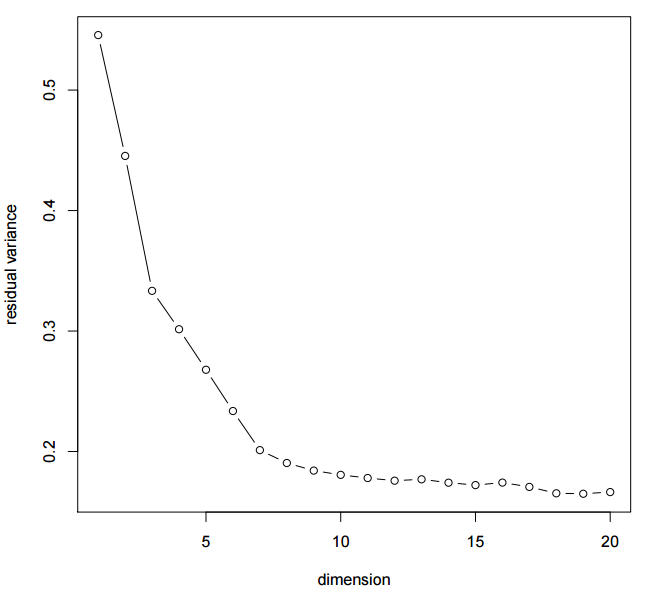
\includegraphics[width=1\linewidth]{iso_resid_var.png}
      \caption{Residual variance not captured by a multidimensional scaling in to $x$ dimensions.}
    \end{subfigure}
    \begin{subfigure}{.47\textwidth}
      \centering
      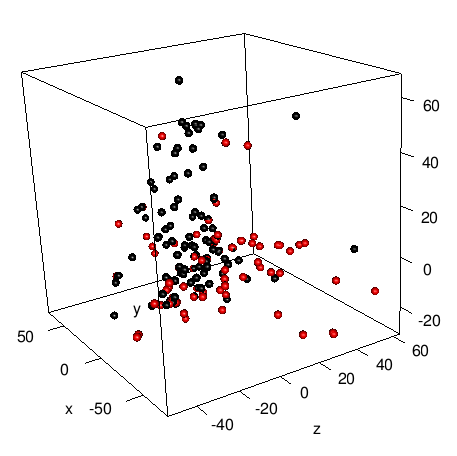
\includegraphics[width=1\linewidth]{isos3d.png}
      \caption{Separation of the data when multidimensional scaling to 3 dimensions.}
    \end{subfigure}
    \caption{Isomap results.}
    \label{fig:isos}
  \end{figure}

  The Isomap function appears to construct the adjacency graph once using the given $k$ and does multidimensional scaling to however-many dimensions we specify. Figure \ref{fig:isos}a depicts the variance of residual information not captured by scaling to 1 through 20 dimensions. Notice that more dimensions is better up until some point where the residual variance does not decrease any more and can even jostle back upward (20 as opposed to 18, for example). For comparison with PCA, I include a point-cloud for the scaling to 3 dimensions. Notice there is a little separation, despite a still relatively high residual variance. To generate this plot yourself, use \texttt{first3isos.R}.

  \subsubsection{Hierarchical clustering}

  The final dimensionality reduction technique I have used is iterative hierarchical clustering. It works as follows:

  \begin{lstlisting}[mathescape]
  1. Each item (CpG) begins in its own group with a variance across $N$ people.
  2. Drop groups with a variance that is below some threshold.
  3. Combine all groups in to one and divide it in to $k$ groups ($k=2$) by
     $k$-means clustering if its `coherence', defined as the average covariance
     between every locus in the group and the group's mean, is not above some
     threshold ($c_{1}$). Repeat $L$ times or until no more groups can be divided.
  4. Compare groups to each other and merge them if the correlation of their
     centers is greater than some cutoff ($c_{2}$).
  \end{lstlisting}

  In some ways this method is more intuitive and interpretable than the others: We take gene loci, make sure that they are varying across our samples, and then combine them in to ``modules'' that vary together. The results are clusters of loci, something biologically meaningful, and the $d$ features for each of the $N$ samples are degrees to which they express those modules.

  \subsection{Learning to distinguish samples based on disease state}

  The last stage on the left of the flow chart is classification. Files beginning with 3s are features-files, literally $N \times d$ tables of numbers that we can use to characterize samples in $d$-dimensional space. They are now quite small and manageable, so we can use use an algorithm to classify them on any local machine.

  In the interest of making a solution that is extremely intuitive, quick to code, and does not require millions of examples, I decided to use a kNN learner, which classifies samples based on which of their neighbors are closest in the $d$-space. \texttt{classify.py} makes use of my \texttt{KNNLearner.py} object as well as the \texttt{numpy} and \texttt{pandas} packages in \texttt{Python 2.7}, so install these. Open the code and look at the upper section where the \texttt{data} is read in; ensure you are reading the data you want and either normalizing it or not normalizing it depending upon your choice. Run the program with \texttt{python classify.py} in a command line pointing to the \texttt{/code} subdirectory.

  If you read the code, you will see there are two loops. The first is to find the best setting for the kNN ``hyperparameter'' $k$. Most machine learners have these kinds of parameters, values you the user have to set in the beginning without much guidance. For neural networks these include the number of layers and the number of hidden neurons per layer. For decision trees there is the max depth and the branching factor. The general rule is to try lots of different hyperparameters to find which ones work best on the training data and then stick with these.

  I use the second loop as part of a ``leave-one-out'' testing scheme. The idea is that we don't have very many samples at all, so to divide the data in to training and testing sets might leave both sets too small. Instead, we can withold a single sample, train a model on the rest, test on that one sample, and repeat for all samples in the data. For an idea of accuracy, the number of models that correctly classified the one left out is divided by the $N$ models created.

  The plot displayed when execution finishes shows three things vs $k$: (blue) the average accuracy of the models on the data on which they were trained, (red) the average accuracy of the models on the data point left out, (green) the acccuracy of a random classifier that just picks `Control' or `Schizo' at a rate proportionate to their occurence in the data (should be about 50\%).

  \begin{figure}[H]
    \centering
    \begin{subfigure}{.33\textwidth}
      \centering
      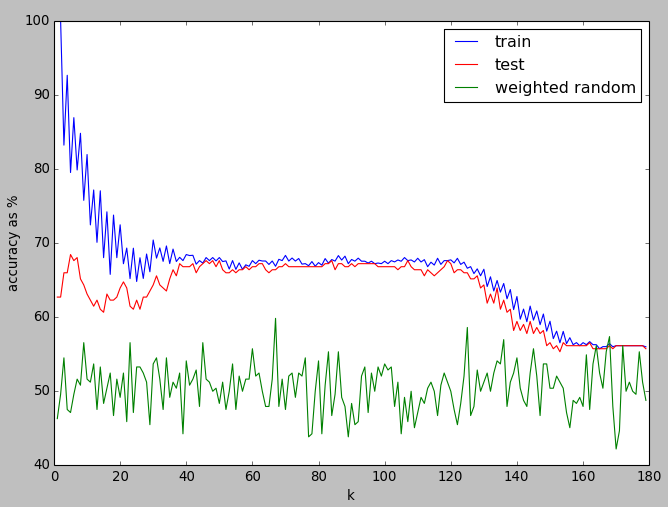
\includegraphics[width=1\linewidth]{3pcs.png}
      \caption{3 PCs}
    \end{subfigure}
    \begin{subfigure}{.33\textwidth}
      \centering
      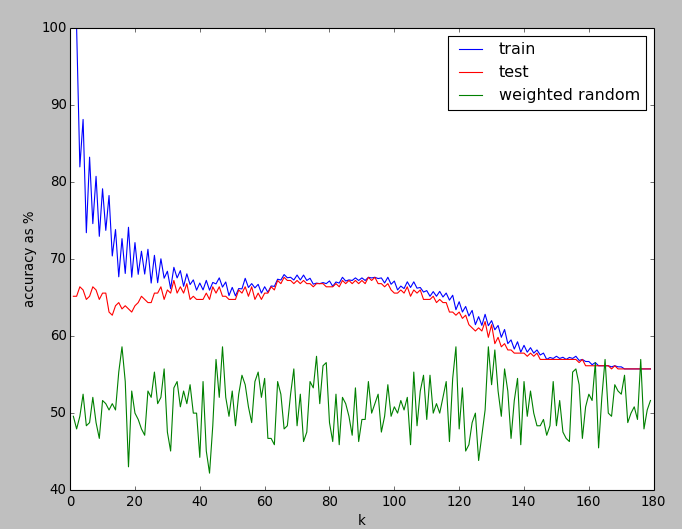
\includegraphics[width=1\linewidth]{10pcs.png}
      \caption{10 PCs}
    \end{subfigure}
    \begin{subfigure}{.32\textwidth}
      \centering
      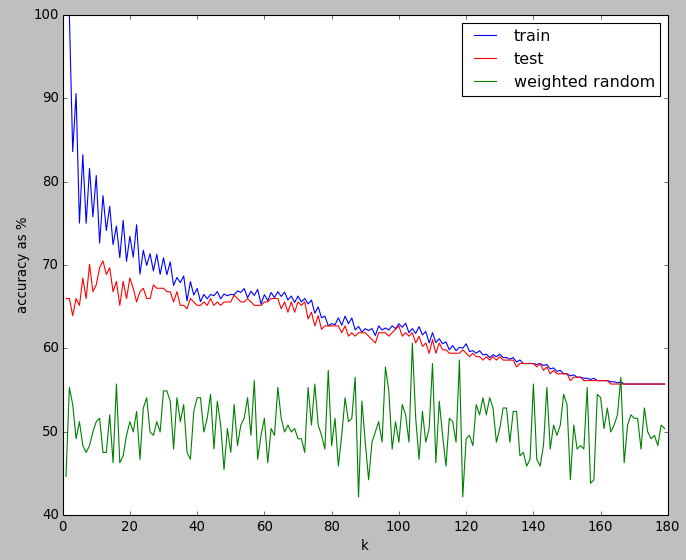
\includegraphics[width=1\linewidth]{10pcsnorm.png}
      \caption{10 normed PCs}
    \end{subfigure}
    \begin{subfigure}{.33\textwidth}
      \centering
      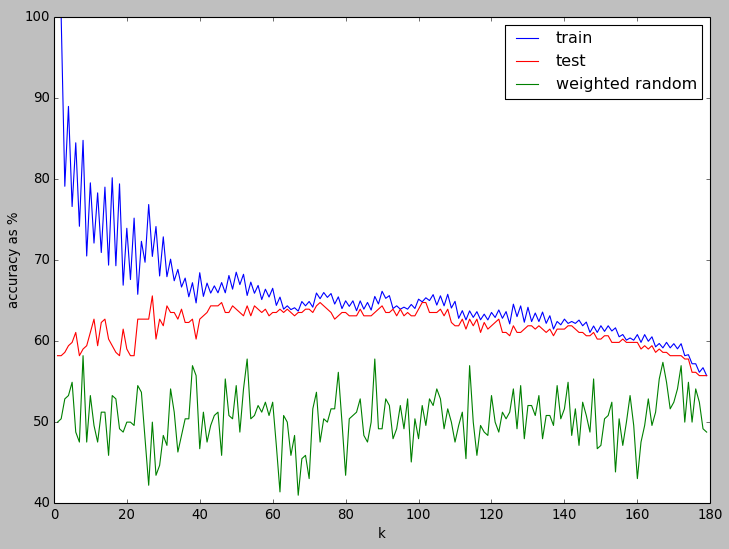
\includegraphics[width=1\linewidth]{3isos.png}
      \caption{3-d isomap features}
    \end{subfigure}
    \begin{subfigure}{.32\textwidth}
      \centering
      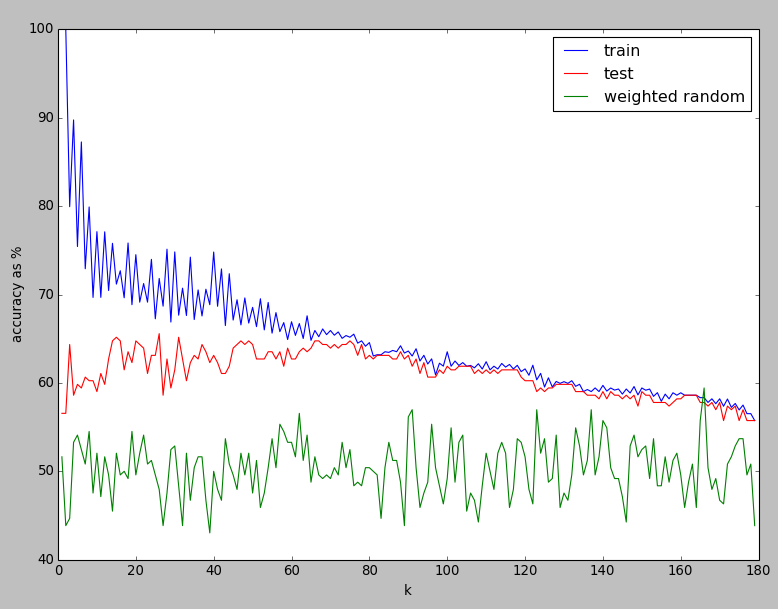
\includegraphics[width=1\linewidth]{10isos.png}
      \caption{10-d isomap features}
    \end{subfigure}
    \begin{subfigure}{.33\textwidth}
      \centering
      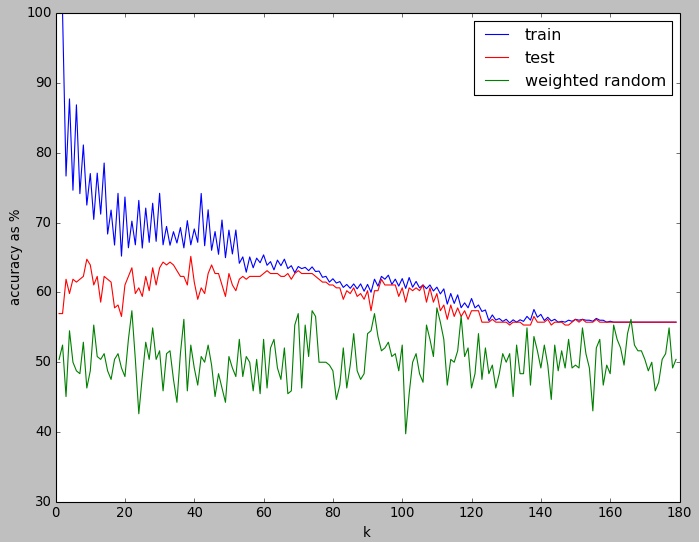
\includegraphics[width=1\linewidth]{10isosnorm.png}
      \caption{10-d normed isomap features}
    \end{subfigure}
    \caption{kNN classifier results.}
    \label{fig:classify}
  \end{figure}

  Figure \ref{fig:classify} displays some results. The upper row makes use of features found via PCA, and the lower row makes use of features found with Isomap. The left column is classifying with 3-dimensional data; the middle column uses 10-dimensional data; and the right column uses 10-dimensional data that has been divided in each dimension by the standard deviation across all points in that dimension (to make the point-cloud more equally stretched in all dimensions, a preprocessing step which is often recommended for kNN).

  Notice a few things:

  \begin{enumerate}
    \item For small $k$, the training accuracy greatly exceeds the testing accuracy. This is called ``overfit'' and happens because whatever model we find to describe the training data does not generalize to the testing data; it is too attuned to the data it has seen. At larger $k$ there is a smoothing effect, so overfit goes away, and the red and blue lines converge.

    \item In all cases the kNN classifier is doing better than random! This means there \textit{appears} to be some signal left in the flattened data. Caution! We have very few data points, so this performance, no better than about 70\%, may be an artefact of some oddities in the small dataset. (See Section \ref{s:future}.) What can say right away given the classifier's imperfect performance is that whatever signal there may be is either not present for all samples, is overwhelmed by noise much of the time, or can not be perfectly-described by the surfaces kNN is finding. (We may need something else \ref{s:future}.)

    \item Norming the data doesn't have much of an effect, aside maybe from marginally depressing the accuracy of a 10-PCA classifier at high $k$ and raising it at lower $k$. (I suspect this is an artefact of our dataset and will not generalize.)

    \item PCA might be a better feature-extraction method than Isomap, as classifiers based on PCA features to do consistently slightly better. Maybe the microarray data actually correlates linearly with disease state.
  \end{enumerate}

  \subsection{Learning to identify progressions}

  So we suspect that there is \textit{at least a little} signal left in the flattened data and that we can see some of it in lower dimension with PCA or Isomap. But what can we do with such a system? Long-term, the chief clinical application is diagnostic: Can we take tissue that is easily accessible (blood, for example), run it through a series of assays, and then use the resulting raw data to determine disease state for a variety of conditions? That sort of technology would require faster, cheaper tests on the wet-lab side and more honed learners on the analytical side, and it's years away.

  Let's rephrase the question ``Can we predict disease state?'' to ``Can we identify the underlying progression of a disease?''. That might allow us to see what the most significant common threads are among diseased individuals and connect them to genes and the like, a much more interesting prospect for biologists. Now let's think like engineers: Can we build a system that can identify a meaningful progression from non-diseased to diseased?

  Fortunately, Dr. Peng Qiu actually built \href{http://pengqiu.gatech.edu/software/SPD/index.html}{the system} in question (already intended for microarray data) and wrote a great paper about it [\ref{r:spd}]. The algorithm, called Sample Progression Discovery (SPD), is, as I understand it, as follows:

  \begin{lstlisting}[mathescape]
  1. Perform Hierarchical Clustering as described above to obtain `gene
     modules' that vary more than some threshold and are highly correlated
     to themselves across samples.
  2. For each gene module:
     a. Place the samples in a space defined by the genes in that module
        at a location based upon their expression of those genes.
     b. Do density-dependent thinning of the samples in that space (only
        necessary when there are far more samples than we have).
     c. Create a Minimum Spanning Tree (MST) between all the remaining
        points in that space with weights proportional to Euclidean
        distance.
     d. Remember the distances between all samples along edges of the MST
        in a distances matrix (where samples that were thinned out get the
        same values as their nearest included neighbor).
  3. Compare the distance matrices generated by different modules in step 2
     to obtain a similarity metric based upon their `earth mover's distance'
     to one another.
  4. Generate a progression-similarity matrix between gene modules using a
     threshold for whether a fit between a module and a tree is significant.
     `0.05 means that, among all the module-tree pairs, the top 5% with most
     significant [smallest] earth mover's distances are considered to `fit
     well with each other''.
  5. Choose a group of gene modules that support a similar progression, and
     construct the MST that describes that common progression.
  6. Perform Multidimensional Scaling to place the samples in 2D according
     to their tree-distances, and draw tree edges to connect them.
  \end{lstlisting}

  Did you understand? Read it again if you have to; it's really brilliant. There is also an outline in the Methods section of the PLoS paper [\ref{r:spd}] that is simultaneously more and less detailed.

  Unlike the methods explored in the last section, which were supervised, SPD is unsupervised, relying only on blind pattern-finding. In order to make sense of the patterns it identifies, we have to overlay information about the samples \textit{post hoc}. I've written a Matlab script called \texttt{ConstructSPDData.m} to read in both flattened data and metadata and save them in a format SPD can understand. To modify which files it reads, change the input strings ($T = ...$, $M = ...$), making sure the data and metadata match.

  Using SPD is not difficult but takes a few steps and can be a bit opaque unless you understand the algorithm. Follow the \href{http://pengqiu.gatech.edu/software/SPD/index.html}{guide} for maximal efficiency. Here are some hickups I ran in to:

  \begin{enumerate}
    \item This software was originally intended for smaller microarrays. As a consequence, 420k is too many loci. Solve this problem by throwing away loci with more than some number of NAs (If the number is $>$0, then the missing values are imputed.) and by throwing away loci with a standard deviation (across samples) below some threshold. You may have to be aggressive, otherwise clustering may not finish or may yield too many modules.
    
    \item I am not actually certain how the iterative Hierarchical Clustering algorithm works. ``Agglomerative'' clustering is only the second half of what I and [\ref{r:spd}] describe.

    \item Ideally, the modules at the end are 50-200 loci, each with a very high coherence (see plots by clicking ``module quality''). But in practise I have found it difficult to obtain modules like this. Either they are of wildly varying sizes (usually a few much much larcher than the others) or there are too many modules, all just above the minimum module size.

    \item Beware too many modules! Computing fits between modules and trees (via earth mover's distance and distance matrices) is $O(n^{2})$ with the number of modules. If $n$ goes much over 100, it will take a very long time to finish.

    \item Dr. Qiu's recommendation is that you vary the percentage of module-tree pairs used to construct the similarity matrix between 5\% and 15\%. The idea is that for a few different values you should see some of the same groups of gene modules making up the bright, highly-correlated blocks. Those groups are what you should enter manually.

    \item If you don't want to do all the computation again, click ``Save Results'' and wait. (It takes a while.) If you want to read the data in the future, use the ``Load result file'' option instead of ``Load raw data''.
  \end{enumerate}

  At the end of this process, clicking ``View Progression'' displays a tree that is constructed to fit the best progression commonly supported by the group of highlighted modules. Clicking the ``Color code according to'' check-box allows you to quickly see whether the progression matches well with any known features as recorded in metadata.

  \begin{figure}[H]
    \centering
    \begin{subfigure}{.95\textwidth}
      \centering
      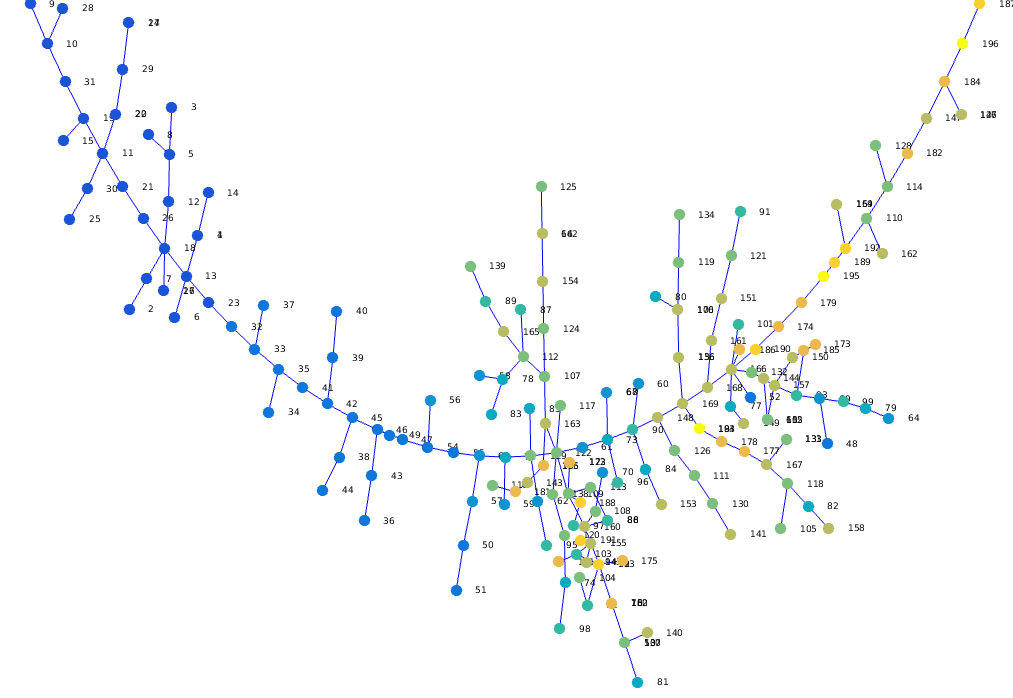
\includegraphics[width=1\linewidth]{control_youth_age.png}
      \caption{Progression with age overlaid.}
    \end{subfigure}
    \begin{subfigure}{.95\textwidth}
      \centering
      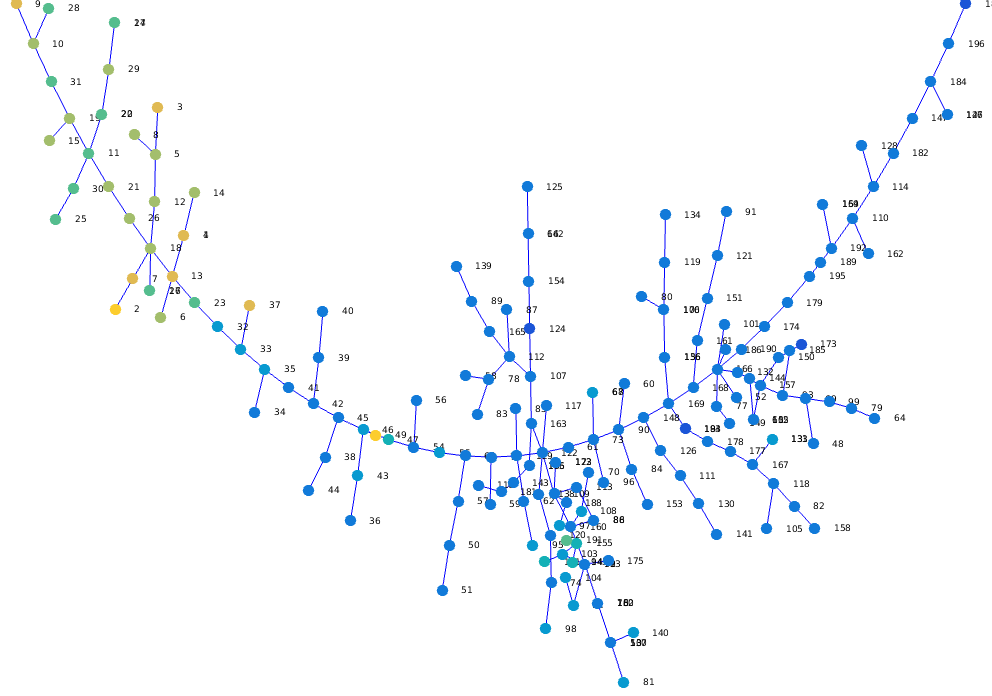
\includegraphics[width=1\linewidth]{control_youth_es.png}
      \caption{Progression with embrionic stem cell concentration overlaid.}
    \end{subfigure}
    \caption{The most significant progression identified by SPD on all not-schizophrenic data (1 module, 1365 loci).}
    \label{fig:spd1}
  \end{figure}

  Figure \ref{fig:spd1} shows SPD's best results. This is on not-flattened data including every sample that is not from a schizophrenic person. Since overlaying age and age-related factors definitely agrees with the identified progression, we know that SPD has found the very obvious epigenetic trends associated with ageing.

  So SPD is not broken. But does it work for identifying more subtle trends? The short answer is that I tried many, many different settings and never witnessed a progression that would diffinitively explain disease state. Figure \ref{fig:spd2} shows a typical example.

  \begin{figure}[H]
    \centering
    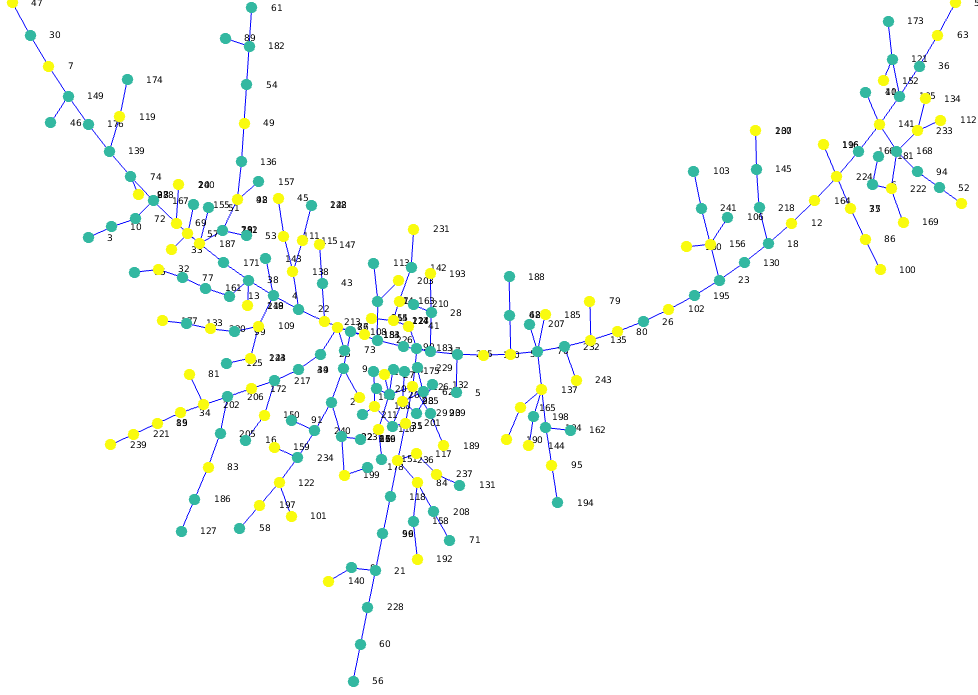
\includegraphics[width=1\linewidth]{sz_control_dx.png}
    \caption{The most substantial progression identified (6 modules, 42 genes) from flattened $>$16yr control and schizophrenic samples with disease state overliad (yellow is control).}
    \label{fig:spd2}
  \end{figure}

  Although SPD can clearly identify progressions due to plate (batch effects) and age when I feed it the processed data (and \textit{maybe} a couple subtle things due to sex and ethnicity, but remember we removed loci we thought would vary much with those factors), it largely fails to find such patterns in the flattened data. This is good news: The flattening process is doing what we want. The bad news is that there appears to be no pattern \textit{strongly} correlated with disease state in any data set. However, there may be some \textit{weak} relationships here, and it may be worth more exploration \ref{s:future}.
 
  \section{The Cluster} \label{cluster}

  In in the interest of not distracting you the reader with too many things at once, I have so far neglected to cover the cluster at a granular level. But I would have liked a compressed introduction myself, and you will need it to carry out the steps in the last section, so I've generously given you this gift.

  If you don't know what a computer cluster is or have never heard of map-reduce, I recommend falling down a Wikipedia rabbit-hole for a few days or reading the original paper from \href{http://research.google.com/archive/mapreduce.html}{Google}. Today's networked computing environments do amazing things, and understanding parallelization can be useful.

  \subsection{File I/O}
  First, open a terminal and type \texttt{ssh pkomarov3@biocluster-6.pace.gatech.edu}, replacing username and cluster name as necessary. I can access bioforce-6, biohimem-6, iw-shared-6, and testflight; you might use different ones. Give your password to log in, and then type \texttt{pwd} to determine the path to your root directory, something like \texttt{/nv/hp10/pkomarov3}. To quit the ssh connection at any time, use \texttt{exit}.

  Next, open nemo (or any other file browser that supports sftp) and type something homologous to \texttt{sftp://pkomarov3@biocluster-6.pace.gatech.edu/nv/hp10/pkomarov3/} in to the url bar. It may require a password the first time and will take you to the 5GB user directory. You can do whatever you want here. I created a \texttt{/code} subdirectory to hold all scripts and job submission (\texttt{.pbs}) files. \texttt{/data} is 200GB of storage that will be saved (unlike the 7TB \texttt{/scratch} which is wiped every 60 days). Be aware that uploading to and downloading from the cloud is slow unless plugged in to LAWN.

  \subsection{Submitting jobs}
  Pbs files are to provide the cluster with job details, because R scripts and such do not contain instructions for this layer. Here is a simple example:

  \begin{verbatim}
  #PBS -N pavelGetResiduals
  #PBS -q iw-shared-6
  #PBS -l nodes=1:ppn=1
  #PBS -l walltime=12:00:00
  #PBS -l mem=20gb

  cd $PBS_O_WORKDIR
  module load R/3.1.0
  Rscript GetResiduals.R
  \end{verbatim}

  \vspace{-3mm}
  Anything beginning with \texttt{\#} is an instruction to the order-processsing node like ``When the job terminates, give me everything the program printed in files named `pavelGetResiduals'.'', ``Submit to the iw-shared-6 queue.'', ``Use 1 node with a minimum of 1 processor each.'', ``Make sure this thing doesn't run more than 12 hours.'', and ``Make sure the nodes have 20GBs of memory.''. \texttt{cd \$PACE\_O\_WORKDIR} ensures the nodes that execute the job are looking in the directory whence a job was submitted (the current directory of the terminal at submit-time). Hereafter follow any instructions a node needs to execute to complete the job.

  To submit a job, use the command \texttt{msub script.pbs} in a terminal sshed to the cluster. If successful, it should print the job number. To cancel the job, use \texttt{qdel <job number>} (for example \texttt{qdel 100200300}). To view the status of a job, use \texttt{qstat | grep <username>}. Q means the job is currently queued and will be run when there is a free node. R means the job is running. C means the job has completed.

  \subsection{Additional libraries} \label{adlib}
  If you require libraries that are not native to whichever code modules you are loading, then you must install them in the cluster. This is done from the command line through an \texttt{ssh} connection. Since PACE is connected to the internet, you can download anything you need to your 5GB user directory. For example, \texttt{Isomap.R} requires the \texttt{RDRToolbox}. To get this library and supporting libraries: (1) Load an R module of your choice (listed in \texttt{/etc/modulefiles/R/} on the PACE node) with a call like \texttt{module load R/3.2.4}. (2) Enter the R environment with \texttt{R}. (3) Get the Bioconductor installer with \texttt{source("https://bioconductor.org/biocLit} \texttt{e.R")}, call \texttt{biocLite("RDRToolbox")}, and answer \texttt{y} to its questions. (4) Make sure your R file has the appropriate \texttt{library(RDRToolbox)} reference. (5) Make sure the corresponding \texttt{.pbs} file is set to load the same version of R that you just used to install the packages.

  Note that the cluster offers more possibility than this. For a full introduction, visit \url{http://www.pace.gatech.edu/getting-started-pace-clusters}.

  \section{Suggested direction and future work items} \label{s:future}

  In the course of this project and in organizing the work well enough to write this document, we ran upon a great many possible paths. That's part of what makes this project exciting. Here are some ideas, a few specific and actionable and a few general:

  \begin{enumerate}
    \item Use better preliminary data. That is, use more reliable data that includes more loci. This would largely solve ``Are we seeing the correct loci?'' and ``What should we do about \texttt{NA}s?''. Right now Paramita is working very hard to generate such data.

    \item Use more data. This one is maybe intractible, because good biological data is currently absurdly expensive to generate. But in order to be able to train a supervised learner like a neural net to distinguished diseased from not-diseased, we fundamentally (see 7.) need tens of thousands, even hundreds of thousands of samples. Keep this theoretical limitation in mind, and try to side-step this problem wherever possible. It may be possibe to do ``boot-strapping'' on a bit less data or to accomplish what you need with a learner that doesn't require so many training examples. It may be possible to pull data from multiple studies, but then you run in to batch effects of the worst possible kind, and we are unsure how to surmount them.

    \item It is possible the linear regression model we used to fit the data and cancel strong methylation effects is not the best option. I am not sure it is advisable to try something else, because the flattened data is so flat that it appears the linear model fits exceedingly well. Plus, Ixa has said that linear models of this sort are the norm, so doing anything else requires biological justification. Depending upon the learner, it might not be necessary or advantageous to flatten the data because doing so undoubtedly deforms features pertaining to disease state. SPD, for example, is intended to find multiple, unrelated, progressions, so we should ideally be able to see one due to age, one due to sex, one due to disease state. Likewise, some learners can be trained to look for subtle cues and ignore broad effects. Consider the options carefully in each new situation.

    \item It is tempting to say that an classifier accuracy of $\approx$68\% when random does no better than $\approx$50\% is a positive result. (Actually, until today I have been saying it is.) But it is important to remember that our $n = 244$, and that is very small. What is the probability this result is just an artefact of the data? How can we prove statistical significance? We need a strong mathematical argument to be able to confidently assert the flattened data is not entirely noise. Only then will the sanity check be complete.

    \item I built units to output $N \times d$ tables of samples versus their features for use with a kNN classifier, but no such unit exists for hierarchical clustering features (to what degrees a sample expresses genes in the various modules). Right now these numbers are just floating mysteriously inside SPD somewhere, and I am not sure how to get them out. I would like to run \texttt{classify.py} on such a features and do a couple of visualizations to get an idea of how useful these features are for sample-separation in the modules-hyperspace. My guess is they will not be as good as those found via PCA or Isomap, but since they have the advantage of being biologically meaningful, maybe the tradeoff is worth something.

    \item To me the results of SPD look random with respect to disease state, but looking random doesn't rigorously imply randomness. I would like to have a mathematical argument that can demonstrate that SPD is definitively not picking up trends that have anything to do with disease state or, stronger, that the patterns are entirely random and warrant no further exploration. You may or may not agree. Certainly SPD is still worth thinking about, but beware apophenia.

    \item Think bigger.

    I am slightly unhappy that kNN seems to be the best algorithm for our classification problem, because kNN is relatively simplistic and is almost always outperformed by other algorithms when there is more data available. Do some thinking about alternatives and how and why and in what suitable ways.

    \vspace{-1mm} \quad Note that the typical path to high performance is by framing a classification or regression problem as optimization of some loss function $f(\theta, x)$ with respect to parameters $\theta$. In supervised, parametric learning (like neural nets), this is done by gradient descent upon reciept of each new $(x,y)$ pair according to:

    $$\theta_{t+1} = \theta_{t} - \lambda \nabla f(\theta(t)), \qquad \nabla f(\theta(t)) = [\frac{\partial f}{\partial \theta_{1}}, \frac{\partial f}{\partial \theta_{2}}, ... \frac{\partial f}{\partial \theta_{n}}]$$

    That is, find the direction (in the parameter-space) that will cause the algorithm to be more likely to output $y$ given $x$, and adjust the parameters by a small step (size $\lambda$) in that direction.
    
    \vspace{-1mm} \quad This explanation leaves out all the best parts. I recommend Andrey Karpathy's \href{http://cs231n.github.io/optimization-2/}{notes} for a more complete explanation of the calculus of backpropagation. But the point is that to make such a scheme work, we have to take lots of steps, and that requires WAY more samples than we have (see 2.).
    
    \vspace{-1mm} \quad Still, we should think about all the possibilities. For example, it seems to me that just as upper-layer `neurons' in Convolutional Neural Networks (CNNs) trained on image data adjust themselves to pick out facial structures or lines in some direction or certain colors in particular sections of an image, a CNN trained on genetic data might come to recognize promoters, enhancers, genes, or even relationships between them.
  \end{enumerate}

  If you find this list lacking, see Dr. Yi. I guarantee she has at least twice as many ideas.

  \section{References}

  \begin{enumerate}
    \item \label{r:jaffe} Jaffe, Andrew E., et al. ``Mapping DNA methylation across development, genotype and schizophrenia in the human frontal cortex.'' Nature neuroscience (2015).
    \item \label{r:spd} Qiu, Peng, Andrew J. Gentles, and Sylvia K. Plevritis. ``Discovering biological progression underlying microarray samples.'' PLoS Comput Biol 7.4 (2011): e1001123.
  \end{enumerate}

\end{document}
